\documentclass[11pt]{report}
\usepackage[utf8]{inputenc}
\usepackage[margin=2.0cm]{geometry}
\usepackage{tikz}
\usepackage{fancyhdr}
\usepackage{xcolor}
\usepackage{minted}
\usepackage{graphicx}
\usepackage[parfill]{parskip}
\usepackage{lscape}
\usepackage{multirow}

\usetikzlibrary{automata, positioning, arrows, fit}

\title{Digital Engineering\\Project Task 3}
\author{Y3890959\\Y3878784}
\date{14th March 2023}

\pagestyle{fancy}
\fancyhead{}
\setlength{\headheight}{14pt}
\fancyhead[L]{Project Task 3}
\fancyhead[R]{Y3890959, Y3878784}
\fancyfoot{}
\fancyfoot[L]{Digital Engineering}
\fancyfoot[R]{\thepage}

\makeatletter
\let\ps@plain\ps@fancy 
\makeatother

\setminted {
    fontsize=\footnotesize,
    frame=single,
}

\begin{document}

\maketitle

\chapter*{Task 3: Handshaking and source-synchronous communication}

\section*{1 - FSM Description}

The FSM will start at IDLE state as usual. When the WRITE button is toggled, the logic should transition the
FSM to WRINST\_REQ state, where the FSM will send the write instruction to the SPI to enter write mode, once
the SPI\_WR\_ACK line goes high, we assume the SPI has received the request however, we cannot assume that the
handshake is finished, therefore we move to the WRINST\_ACK state, where the FSM waits for the SPI's ACK
line to go back low in this FSM state, the write request line is pulled low from high. Once WR ACK goes low,
the FSM transitions to the next state, WADDR1\_REQ. As the address vector is 24-bits wide, there needs to be 3
states to trasmit all the data due to the data line being 1-byte wide, furthermore, as the handshaking is only
complete when the WR ACK line goes low, we end up with 3 pairs of states; WADDR*\_REQ and WADDR*\_ACK. Once
all bytes of the address has been sent, the logic waits in the WRHOLD state for the user to set the switches
to their desired value and to press the ENTER button. When ENTER is toggled, the FSM increments the INPT\_CNT 
which is an up-down counter, then performs a write request passing the switch value in the data bus, once the
SPI acknowledges and the handshake completes, the FSM returns to WRHOLD. From WRHOLD, when the WRITE button i
toggled without writing any values, then the FSM goes to IDLE, if values have been written and write mode it
exited, then the FSM moves to the RDHOLD state. In RDHOLD, the logic waits for the user to enter read mode by
pressing the READ button. When that button is toggled, the read instruction, RDINST, is sent with two states
(just like WRINST), the 24-bit address is sent a byte at a time, then the logic reaches the RDOUTP\_REQ state,
where a RD req. is sent to the SPI then the RDOUTP\_ACK where we wait for the handshake to finish. After that
we display the read value using the LEDs. Each time a value is output, the INPT\_CNT is decremented. The FSM
cycles through RDOUTP REQ, ACK, and LEDOUT until all values previously written have been read, as soon as that
condition is met, the logic returns to the IDLE state. There is a up-only counter called DISP\_CNT which is
used to add a delay of 1 second after each LED output has been displayed in the LEDOUT state, this is for
improved readability for the user. The FSM state diagram is shown on the next page.


\textbf{
NOTE: although not shown in the FSM state diagram (due to there not being enough space), when the RESET
button is toggled, the FSM logic will return back to IDLE and reinitialise, ready to restart, regardless
of what state it's in when RESET is pressed.
}

\begin{figure} % ’ht’ tells LaTeX to place the figure ’here’ or at the top of the page
\centering % centers the figure
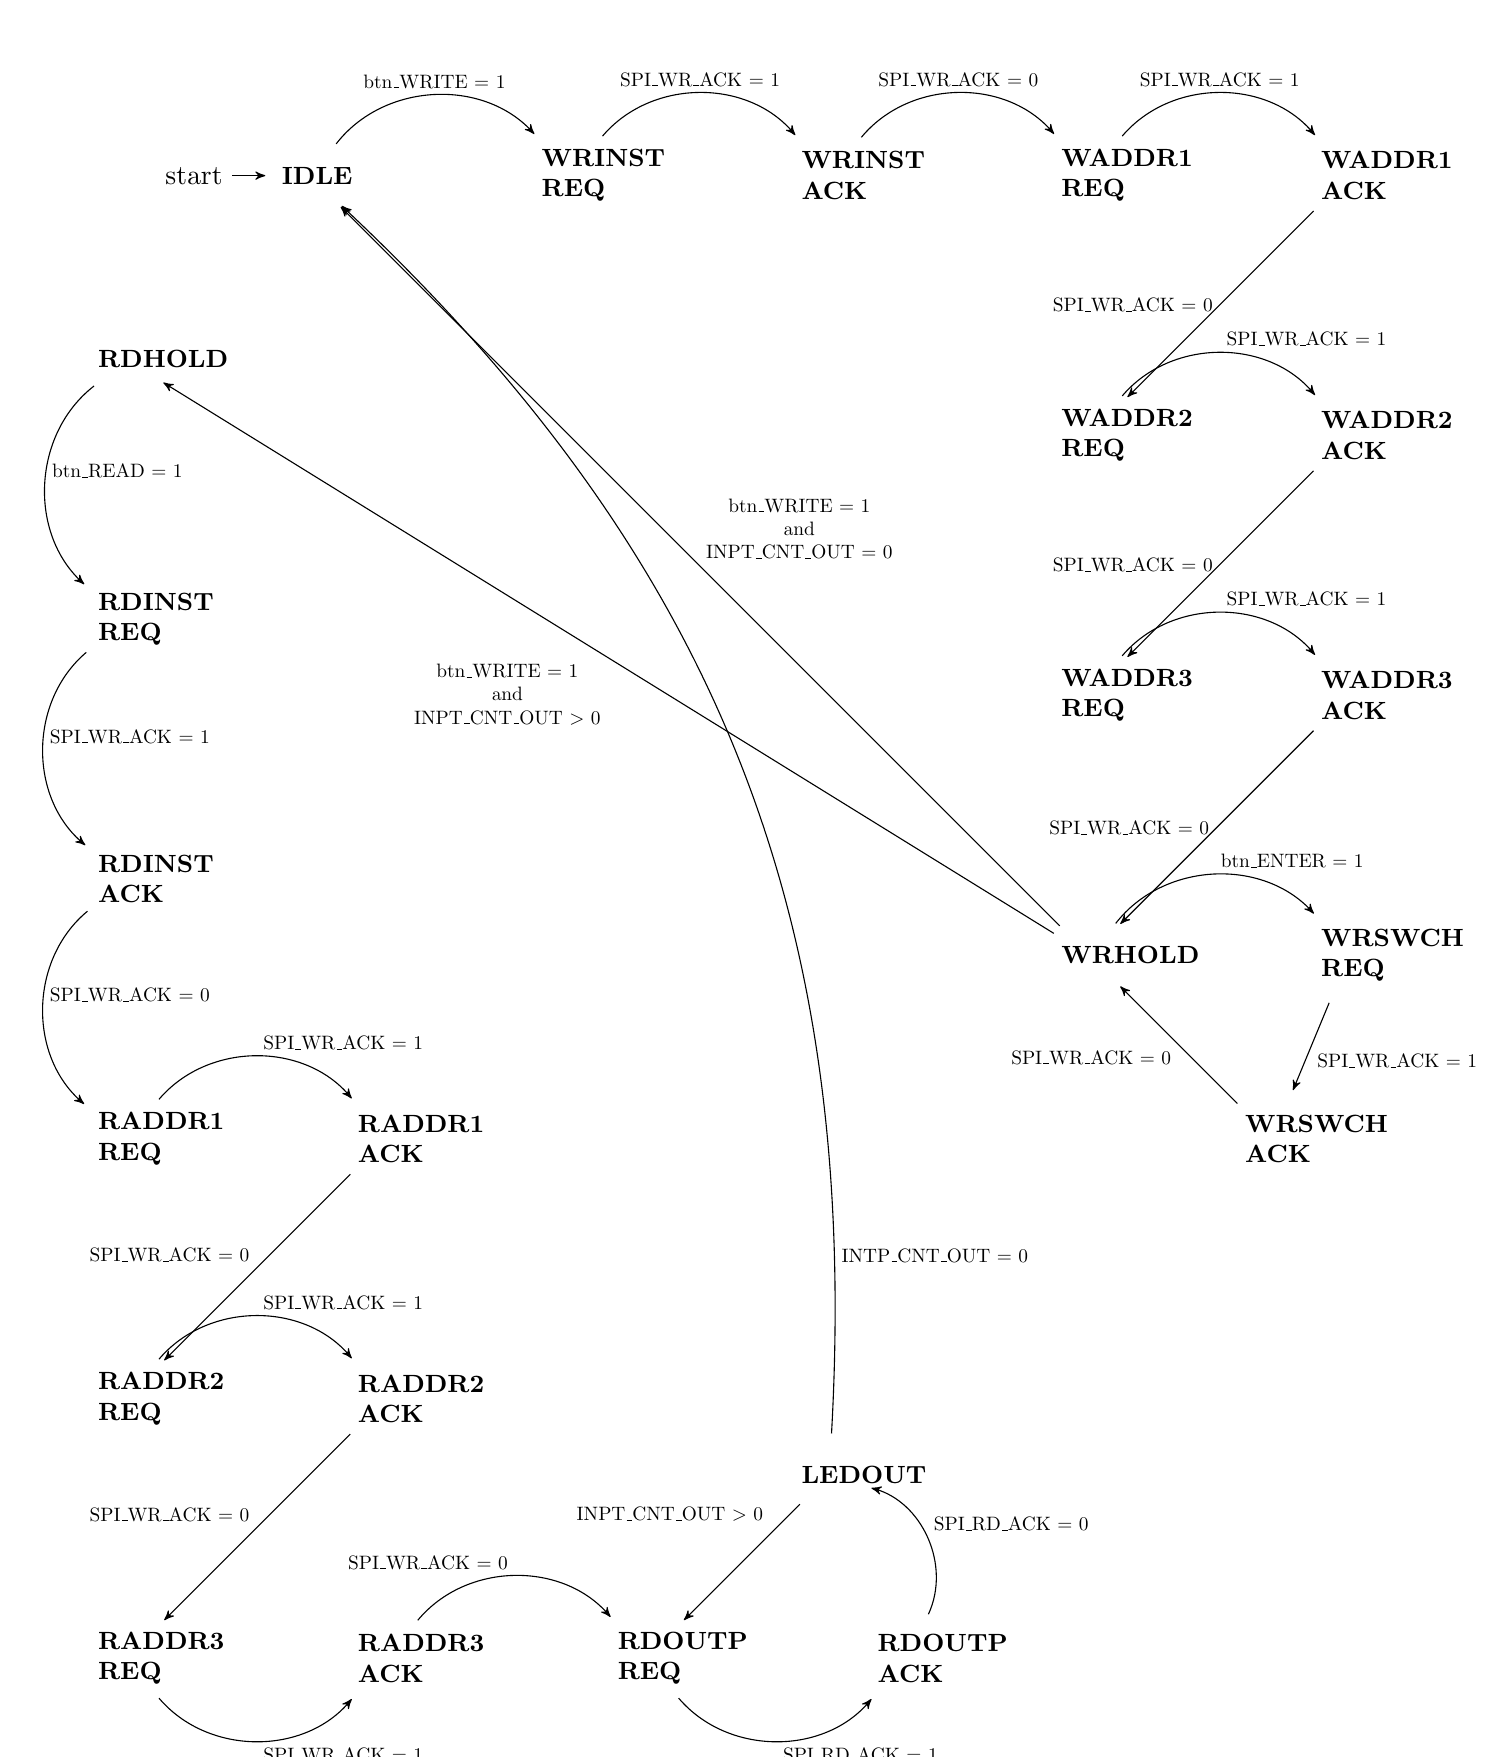
\begin{tikzpicture}[->,>=stealth',shorten >=1pt,auto,node distance=3.3cm]
       \tikzstyle{every state}=[draw=none,text=black,text width=2em,text centered,font=\small]

       \node[initial,state] (A)              {\textbf{IDLE}};;

       \node[state]         (B) [right of=A] {\textbf{WRINST\\REQ}};
       \node[state]         (C) [right of=B] {\textbf{WRINST\\ACK}};

       \node[state]         (D) [right of=C] {\textbf{WADDR1\\REQ}};
       \node[state]         (E) [right of=D] {\textbf{WADDR1\\ACK}};

       \node[state]         (F) [below of=D] {\textbf{WADDR2\\REQ}};
       \node[state]         (G) [right of=F] {\textbf{WADDR2\\ACK}};

       \node[state]         (H) [below of=F] {\textbf{WADDR3\\REQ}};
       \node[state]         (I) [right of=H] {\textbf{WADDR3\\ACK}};

       \node[state]         (J) [below of=H] {\textbf{WRHOLD}};
       \node[state]         (K) [right of=J] {\textbf{WRSWCH\\REQ}};
       \node[state]         (L) [below right of=J] {\textbf{WRSWCH\\ACK}};


       \node[state]         (M) [below left of=A] {\textbf{RDHOLD}};
       \node[state]         (N) [below of=M] {\textbf{RDINST\\REQ}};
       \node[state]         (O) [below of=N] {\textbf{RDINST\\ACK}};

       \node[state]         (P) [below of=O] {\textbf{RADDR1\\REQ}};
       \node[state]         (Q) [right of=P] {\textbf{RADDR1\\ACK}};

       \node[state]         (R) [below of=P] {\textbf{RADDR2\\REQ}};
       \node[state]         (S) [right of=R] {\textbf{RADDR2\\ACK}};

       \node[state]         (T) [below of=R] {\textbf{RADDR3\\REQ}};
       \node[state]         (U) [right of=T] {\textbf{RADDR3\\ACK}};

       \node[state]         (V) [right of=U] {\textbf{RDOUTP\\REQ}};
       \node[state]         (W) [right of=V] {\textbf{RDOUTP\\ACK}};
       \node[state]         (X) [above right of=V] {\textbf{LEDOUT}};

       \path (A) edge [above, bend left=50]  node[align=center, scale=0.7] {btn\_WRITE = 1} (B)
             (B) edge [above, bend left=50]  node[align=center, scale=0.7] {SPI\_WR\_ACK = 1} (C)
             (C) edge [above, bend left=50]  node[align=center, scale=0.7] {SPI\_WR\_ACK = 0} (D)
             (D) edge [above, bend left=50]  node[align=center, scale=0.7] {SPI\_WR\_ACK = 1} (E)
             (E) edge [left]                 node[align=center, scale=0.7] {SPI\_WR\_ACK = 0} (F)
             (F) edge [above right, bend left=50]  node[align=center, scale=0.7] {SPI\_WR\_ACK = 1} (G)
             (G) edge [left]                 node[align=center, scale=0.7] {SPI\_WR\_ACK = 0} (H)
             (H) edge [above right, bend left=50]  node[align=center, scale=0.7] {SPI\_WR\_ACK = 1} (I)
             (I) edge [left]                 node[align=center, scale=0.7] {SPI\_WR\_ACK = 0} (J)
             (J) edge [above right, bend left=50]  node[align=center, scale=0.7] {btn\_ENTER = 1} (K)
             (K) edge                              node[align=center, scale=0.7] {SPI\_WR\_ACK = 1} (L)
             (L) edge                              node[align=center, scale=0.7] {SPI\_WR\_ACK = 0} (J)
             (J) edge [above right] node[align=center, scale=0.7] {btn\_WRITE = 1\\and\\INPT\_CNT\_OUT = 0} (A)
             (J) edge [below left] node[align=center, scale=0.7] {btn\_WRITE = 1\\and\\INPT\_CNT\_OUT $>$ 0} (M)
             (M) edge [above right, bend right=50] node[align=center, scale=0.7] {btn\_READ = 1} (N)
             (N) edge [above right, bend right=50] node[align=center, scale=0.7] {SPI\_WR\_ACK = 1} (O)
             (O) edge [above right, bend right=50] node[align=center, scale=0.7] {SPI\_WR\_ACK = 0} (P)
             (P) edge [above right, bend left=50] node[align=center, scale=0.7] {SPI\_WR\_ACK = 1} (Q)
             (Q) edge [above left] node[align=center, scale=0.7] {SPI\_WR\_ACK = 0} (R)
             (R) edge [above right, bend left=50] node[align=center, scale=0.7] {SPI\_WR\_ACK = 1} (S)
             (S) edge [above left] node[align=center, scale=0.7] {SPI\_WR\_ACK = 0} (T)
             (T) edge [below right, bend right=50] node[align=center, scale=0.7] {SPI\_WR\_ACK = 1} (U)
             (U) edge [above left, bend left=50] node[align=center, scale=0.7] {SPI\_WR\_ACK = 0} (V)
             (V) edge [below right, bend right=50] node[align=center, scale=0.7] {SPI\_RD\_ACK = 1} (W)
             (W) edge [above right, bend right=50] node[align=center, scale=0.7] {SPI\_RD\_ACK = 0} (X)
             (X) edge [below right, bend right=25] node[align=center, scale=0.7, yshift=-250pt, xshift=50pt] {INTP\_CNT\_OUT = 0} (A)
             (X) edge [left] node[align=center, scale=0.7, yshift=25pt, xshift=15pt] {INPT\_CNT\_OUT $>$ 0} (V);
\end{tikzpicture}
\caption{FSM state graph}
\end{figure}

\begin{landscape}
    \begin{table}
    \centering
    \resizebox{\columnwidth}{!}{%
    \begin{tabular}{|l|l|l|l|l|l|l|l|l|l|l|}
    \hline
    \textbf{STATE} &
      \textit{\textbf{EN\_SPI}} &
      \textit{\textbf{SPI\_WR\_REQ}} &
      \textit{\textbf{SPI\_RD\_REQ}} &
      \textit{\textbf{DATA\_TO\_SPI}} &
      \textit{\textbf{INPT\_CNT\_RST}} &
      \textit{\textbf{INPT\_CNT\_EN\_UP}} &
      \textit{\textbf{INPT\_CNT\_EN\_DOWN}} &
      \textit{\textbf{DISP\_CNT\_RST}} &
      \textit{\textbf{DISP\_CNT\_EN}} &
      \textit{\textbf{LEDS}} \\ \hline
    IDLE &
      0 &
      0 &
      0 &
      00000000 &
      1 &
      0 &
      0 &
      1 &
      0 &
      00000000 \\ \hline
    \begin{tabular}[c]{@{}l@{}}WRINST\_REQ\\ RDINST\_REQ\end{tabular} &
      1 &
      1 &
      0 &
      \begin{tabular}[c]{@{}l@{}}WR -\textgreater 00000010\\ RD -\textgreater 00000011\end{tabular} &
      0 &
      0 &
      0 &
      0 &
      0 &
      00000000 \\ \hline
    \begin{tabular}[c]{@{}l@{}}WADDR1\_REQ\\ WADDR2\_REQ\\ WADDR3\_REQ\\ RADDR1\_REQ\\ RADDR2\_REQ\\ RADDR3\_REQ\\ WRSWCH\_REQ\end{tabular} &
      1 &
      1 &
      0 &
      \begin{tabular}[c]{@{}l@{}}ADDR1 -\textgreater SRAM\_ADDRESS(23 : 16)\\ ADDR2 -\textgreater SRAM\_ADDRESS(15 : 8)\\ ADDR3 -\textgreater SRAM\_ADDRESS(7 : 0)\\ WRSWCH -\textgreater SWITCHES\end{tabular} &
      0 &
      0 &
      0 &
      0 &
      0 &
      \begin{tabular}[c]{@{}l@{}}WRSWCH -\textgreater INPT\_CNT\_OUT\\ else -\textgreater 00000000\end{tabular} \\ \hline
    \begin{tabular}[c]{@{}l@{}}WRINST\_ACK\\ RDINST\_ACK\\ WADDR1\_ACK\\ WADDR2\_ACK\\ WADDR3\_ACK\\ RADDR1\_ACK\\ RADDR2\_ACK\\ RADDR3\_ACK\\ RDOUTP\_ACK\\ WRSWCH\_ACK\end{tabular} &
      1 &
      0 &
      0 &
      00000000 &
      0 &
      0 &
      0 &
      0 &
      0 &
      \begin{tabular}[c]{@{}l@{}}WRSWCH -\textgreater INPT\_CNT\_OUT\\ else -\textgreater 00000000\end{tabular} \\ \hline
    WRHOLD &
      1 &
      0 &
      0 &
      00000000 &
      0 &
      \begin{tabular}[c]{@{}l@{}}1 when ENTER = 1 and\\ INPT\_CNT\_OUT \textless input\_limit\end{tabular} &
      0 &
      0 &
      0 &
      INPT\_CNT\_OUT \\ \hline
    RDHOLD &
      0 &
      0 &
      0 &
      00000000 &
      0 &
      0 &
      0 &
      0 &
      0 &
      00000000 \\ \hline
    RDOUTP\_REQ &
      1 &
      0 &
      1 &
      00000000 &
      0 &
      0 &
      0 &
      0 &
      0 &
      00000000 \\ \hline
    LEDOUT &
      1 &
      0 &
      0 &
      00000000 &
      0 &
      0 &
      1 when DISP\_CNT\_OUT = 0 &
      0 &
      1 &
      DATA\_FROM\_SPI \\ \hline
    \end{tabular}%
    }
    \caption{FSM table of outputs}
    \end{table}
\end{landscape}







\section*{2 - VHDL Entity Code}

\subsection*{STUDENT\_AREA Entity - Where the FSM Logic Lives}
\inputminted{vhdl}{../../../DE_Project_T3/DE_Project_T3.srcs/sources_1/imports/DigEng_Proj_T3_model/STUDENT_AREA.vhd}

\newpage

\subsection*{INPT\_CNT Entity - The Up-Down Counter I Made}
\inputminted{vhdl}{../../../DE_Project_T3/DE_Project_T3.srcs/sources_1/new/Param_Counter_UpDown.vhd}

\newpage

\section*{3 - VHDL Testbench Code}
\inputminted{vhdl}{../../../DE_Project_T3/DE_Project_T3.srcs/sim_1/imports/DigEng_Proj_T3_model/TOP_LEVEL_tb.vhd}

\newpage

\section*{4 - Behavioural Simulation}

\subsection*{Waveform 1: Global Reset \& Initialisation Showing Output}
\begin{figure}[H]
    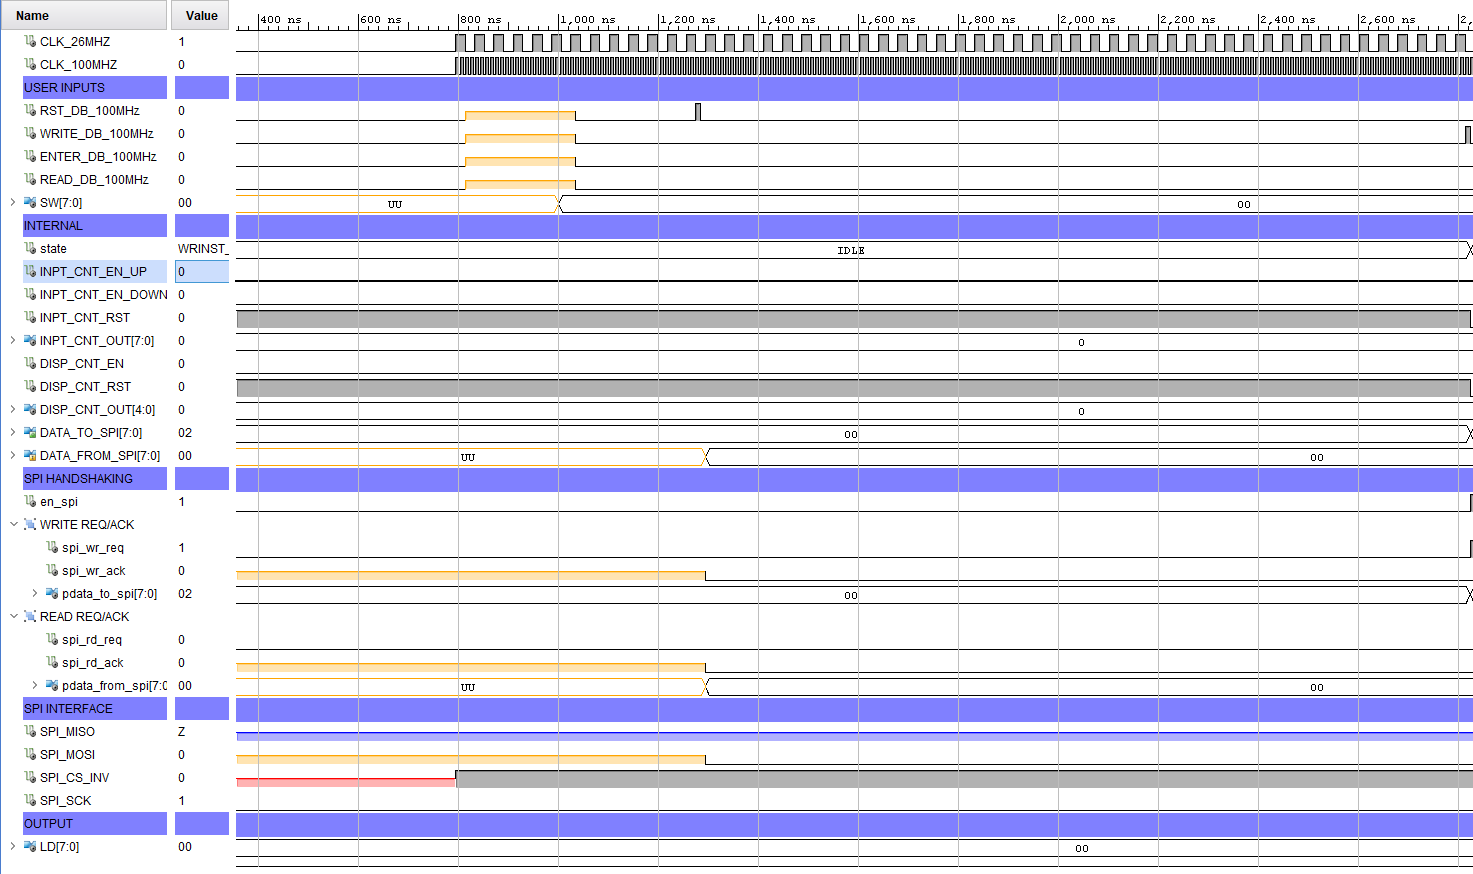
\includegraphics[width=\columnwidth]{Assets/GlobalReset.png}
\end{figure}

Above shows the global Reset \& initialisation: All inputs are initialised to zero, followed by a reset button click.

\subsection*{Waveform 2: Test 1}
\begin{figure}[H]
    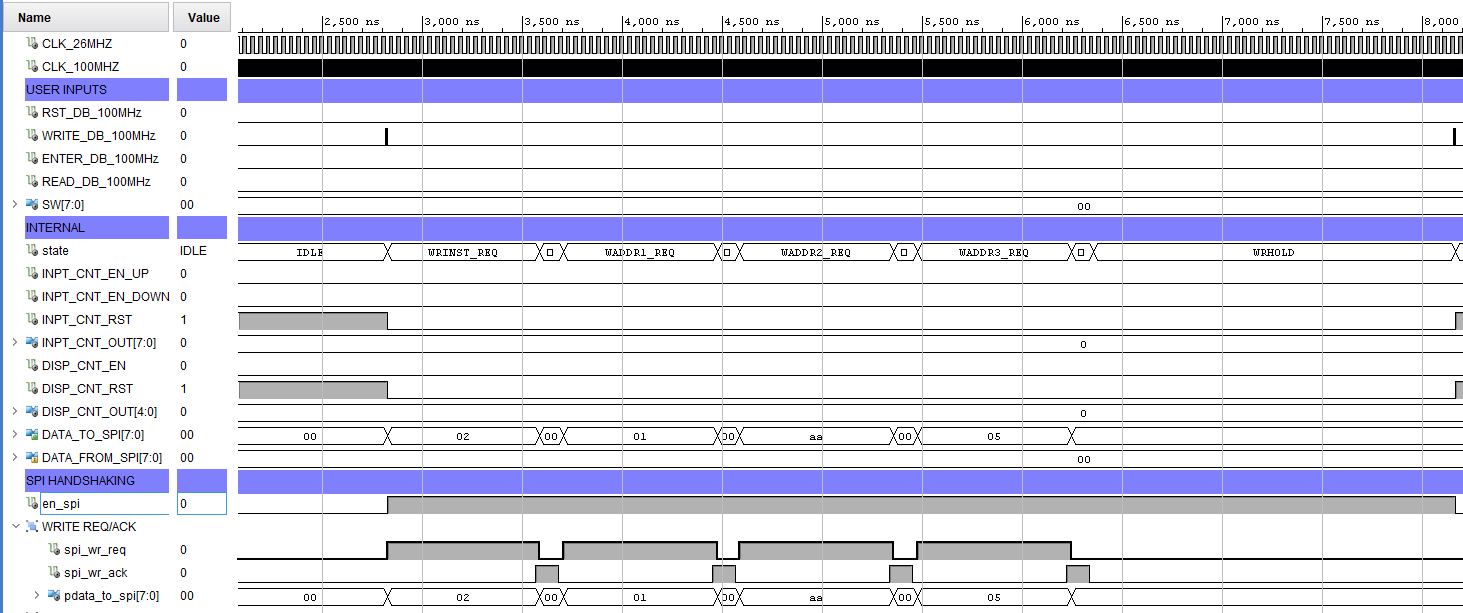
\includegraphics[width=\columnwidth]{Assets/Test1.PNG}
\end{figure}

Waveform 2 shows the code entering `WRITE' mode by pressing the write button, ensure all handshaking aspects of the `SPI' are working correctly, mainly SPI enables, requests are sent, acknowledgements are received and the correct data is sent.

\subsection*{Waveform 3: Test 2}
\begin{figure}[H]
    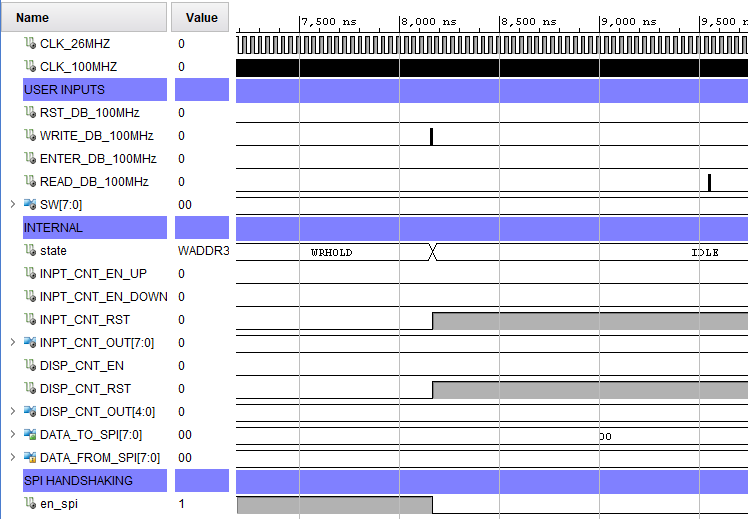
\includegraphics[width=\columnwidth]{Assets/Test2.PNG}
\end{figure}

Waveform 3 follows from Test 1. It begins by exiting `WRITE' mode by toggling the write button. The logic should be able to deactivate the SPI and return back to `IDLE' state.

\subsection*{Waveform 4: Test 3}
\begin{figure}[H]
    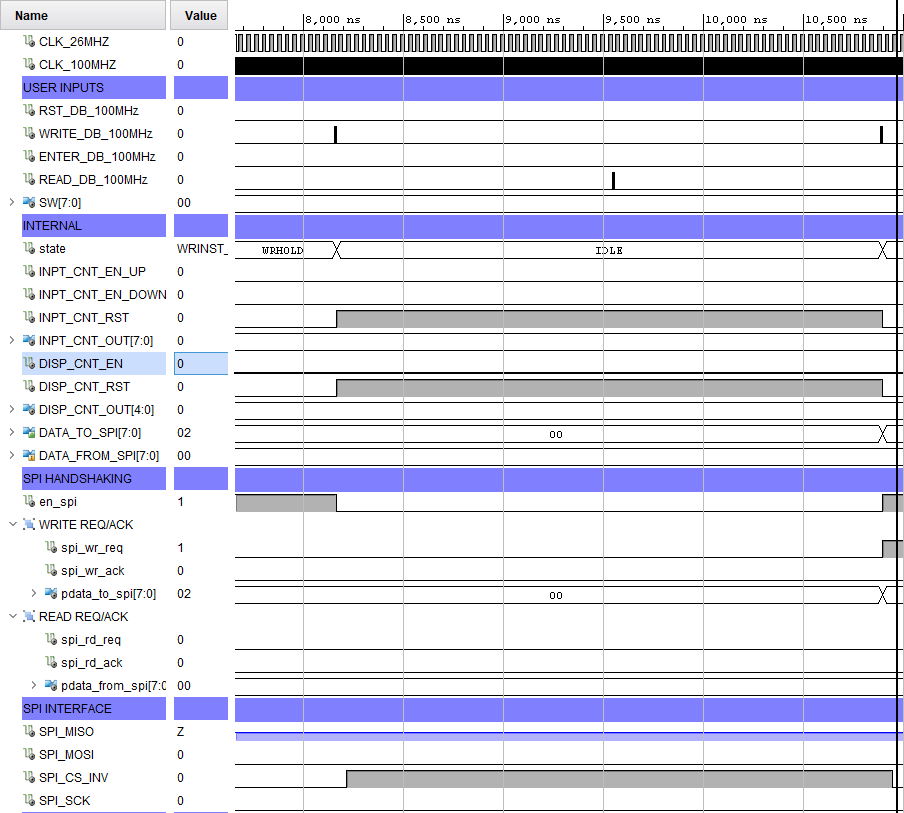
\includegraphics[width=\columnwidth]{Assets/Test3.PNG}
\end{figure}

Toggle the `READ' button to try to enter read mode. This is be blocked by the logic as you can only enter read mode after storing 1 or more values into the `SRAM' in the write mode.

\subsection*{Waveform 5: Test 4\_1}
\begin{figure}[H]
    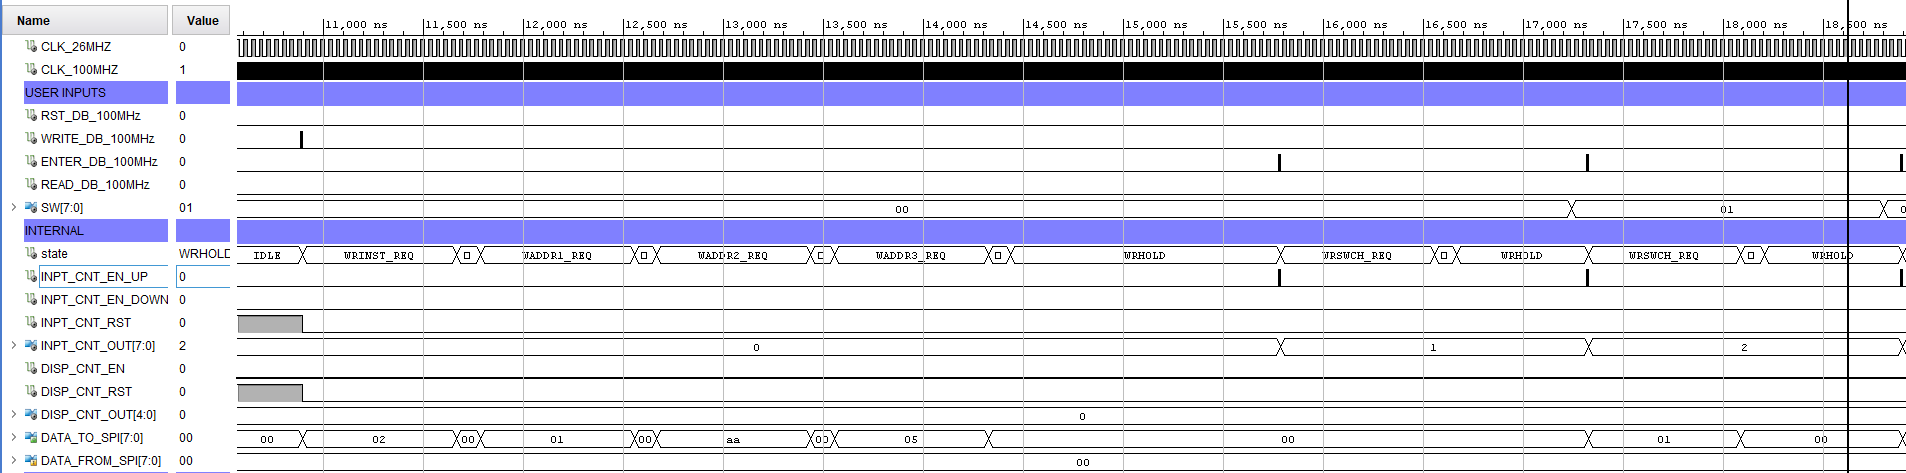
\includegraphics[width=\columnwidth]{Assets/Test4_1.PNG}
\end{figure}

\subsection*{Waveform 6: Test 4\_2}
\begin{figure}[H]
    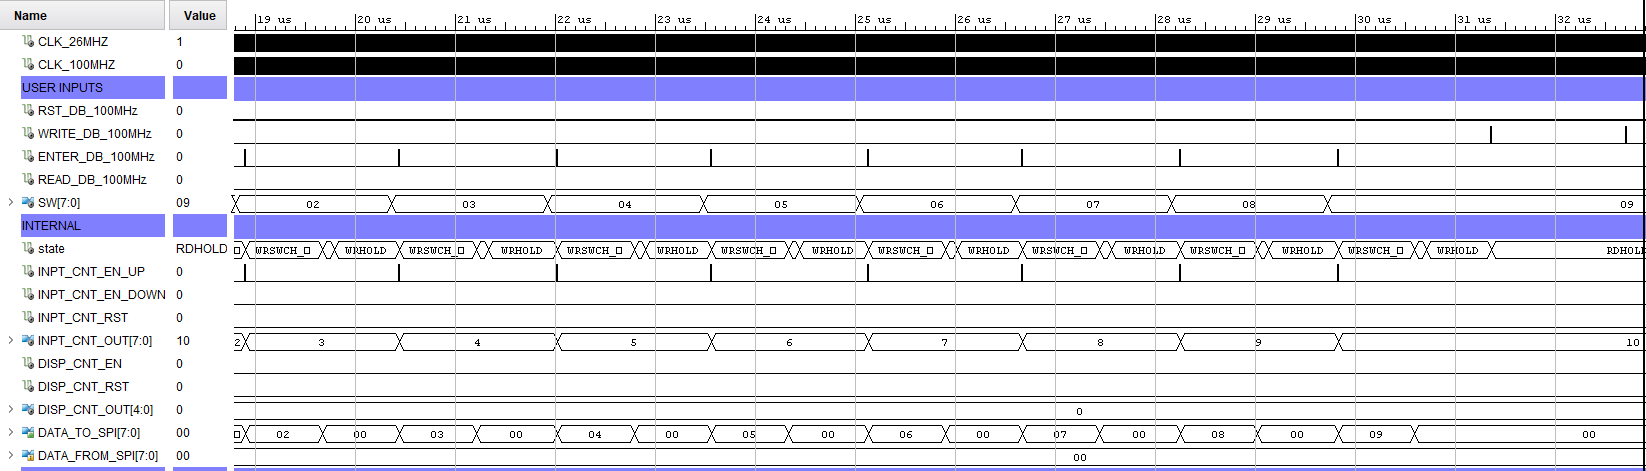
\includegraphics[width=\columnwidth]{Assets/Test4_2.PNG}
\end{figure}

\subsection*{Waveform 7: Test 4\_3}
\begin{figure}[H]
    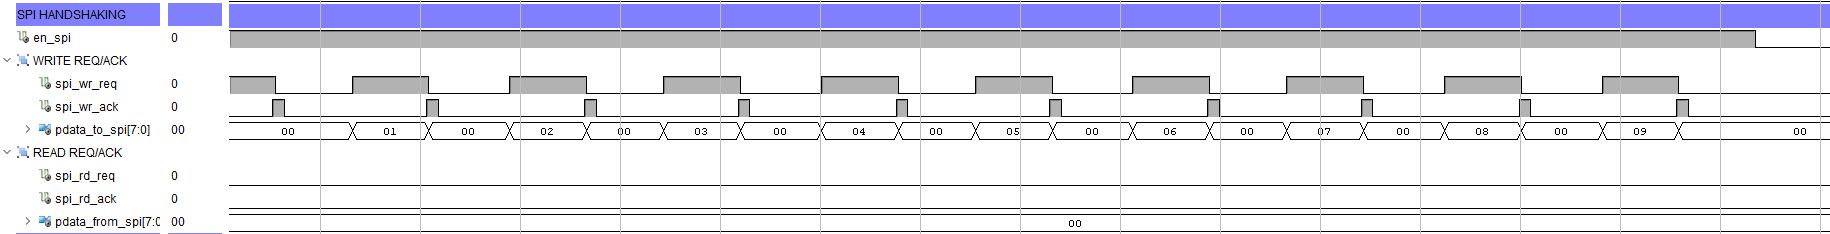
\includegraphics[width=\columnwidth]{Assets/Test4_3.PNG}
\end{figure}

Waveforms 5, 6 and 7 show a follow on from TEST 2, toggle the write button again to enter `WRITE' mode, then store 10 switch values, starting from h"00" and incrementing by 1 each time. Then exit WRITE mode in preparation for the next test. This test should verify that the SPI handshaking logic works when writing data to the SRAM.

\subsection*{Waveform 8: Test 5}
\begin{figure}[H]
    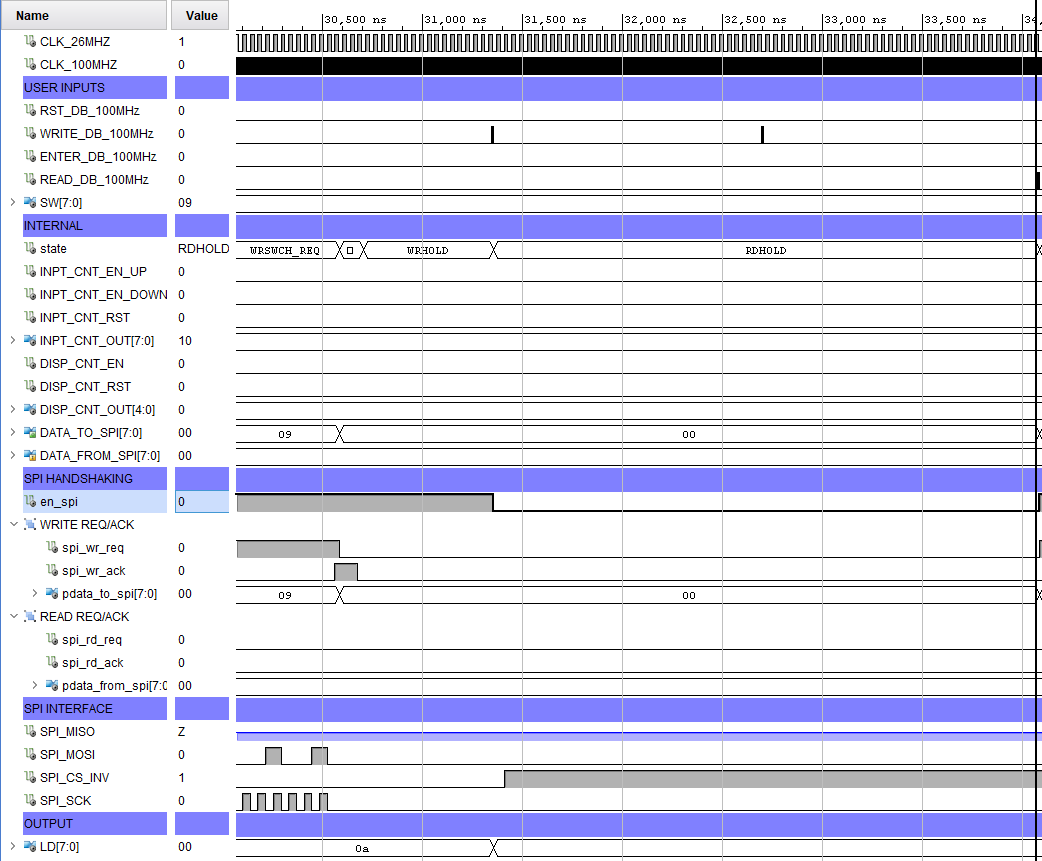
\includegraphics[width=\columnwidth]{Assets/Test5.PNG}
\end{figure}

The above waveform shows a toggle of the `WRITE' button to try to enter write mode again. This is blocked by the logic which prevents write mode to be entered after writing 1 or more values and exiting beforehand.

\subsection*{Waveform 9: Test 6\_1}
\begin{figure}[H]
    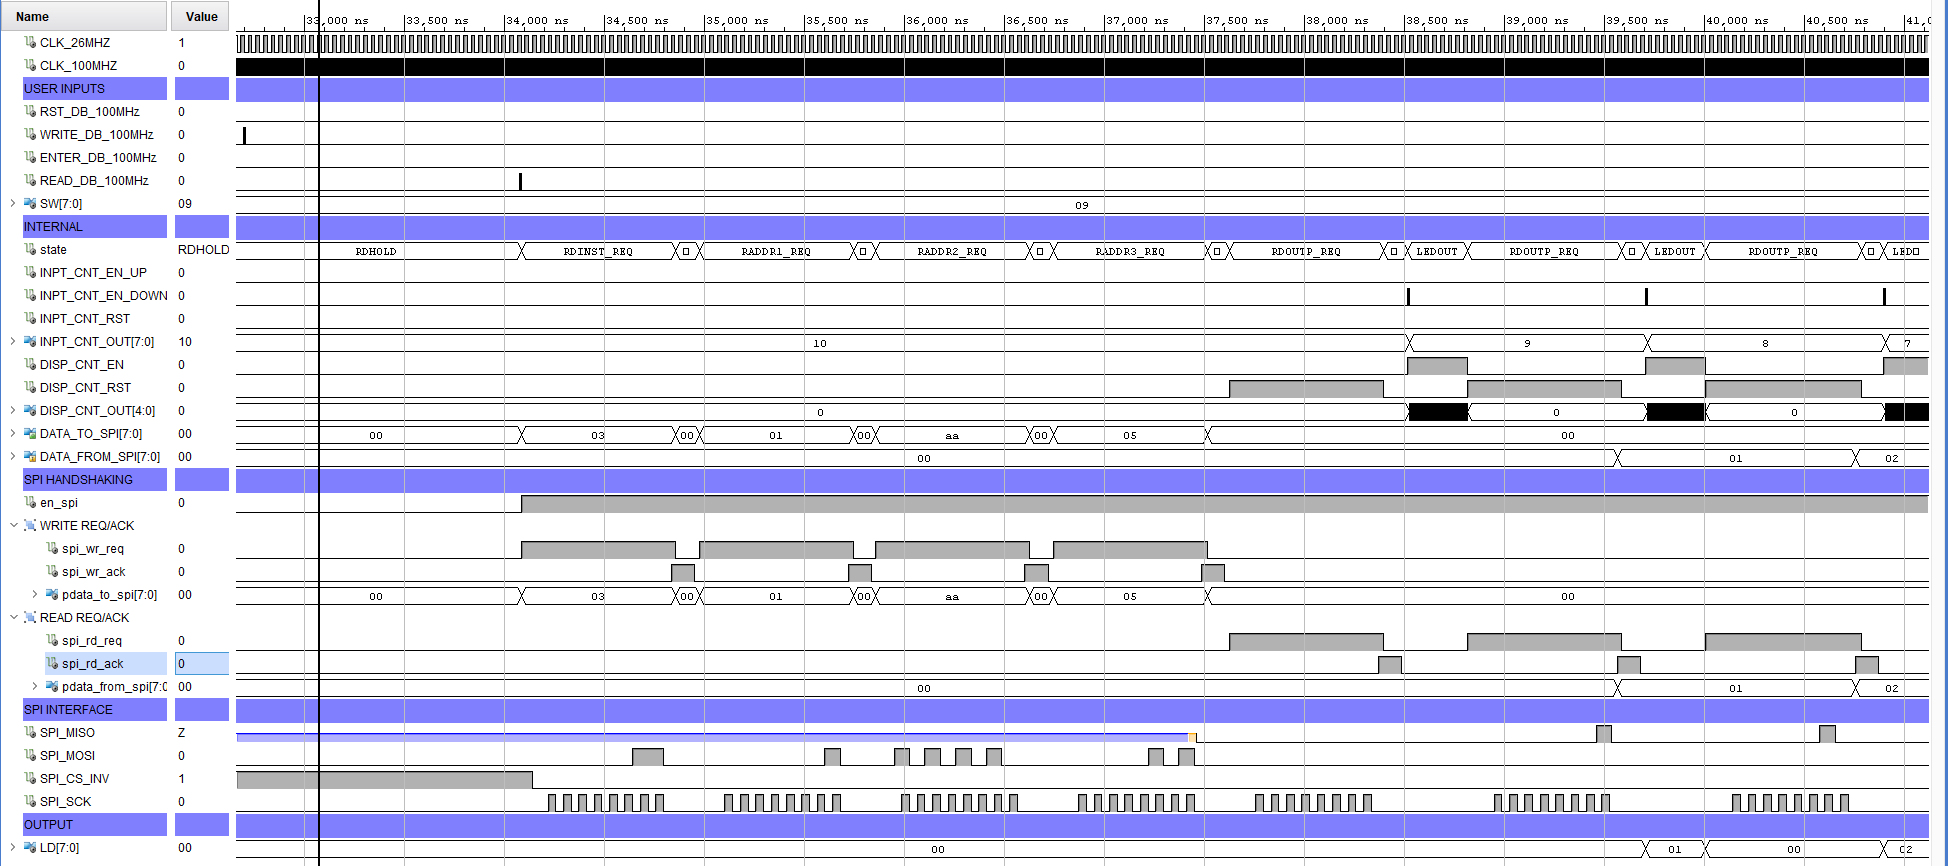
\includegraphics[width=\columnwidth]{Assets/Test6_1.PNG}
\end{figure}

\subsection*{Waveform 10: Test 6\_2}
\begin{figure}[H]
    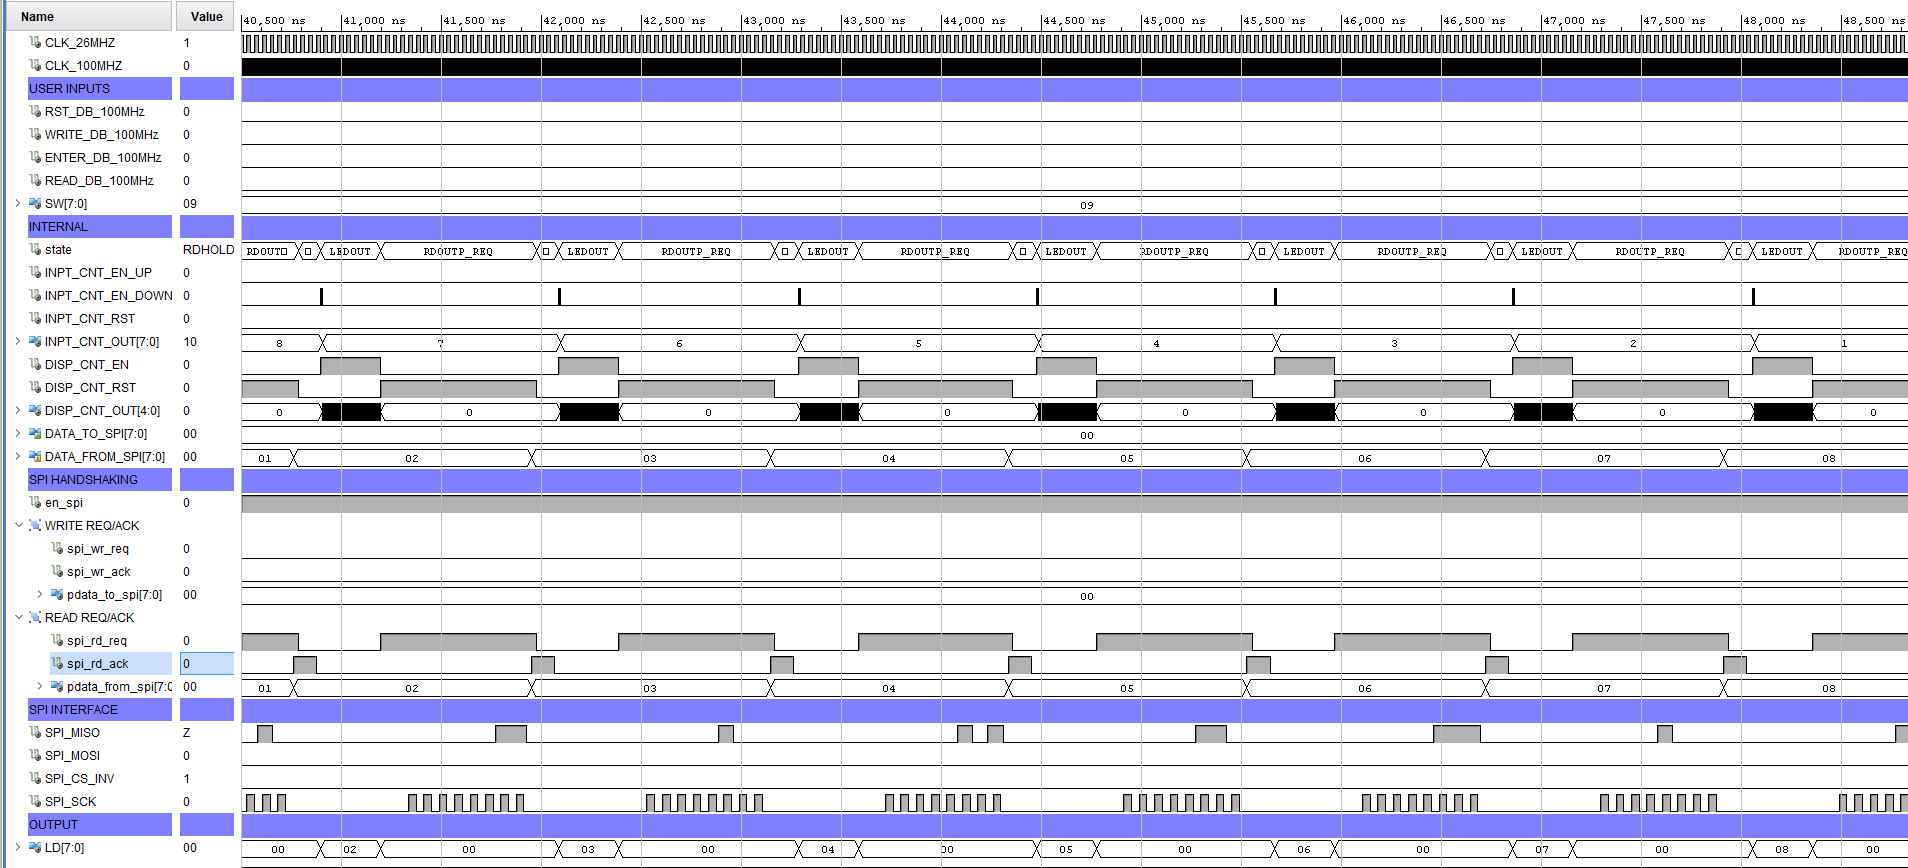
\includegraphics[width=\columnwidth]{Assets/Test6_2.PNG}
\end{figure}

\subsection*{Waveform 11: Test 6\_3}
\begin{figure}[H]
    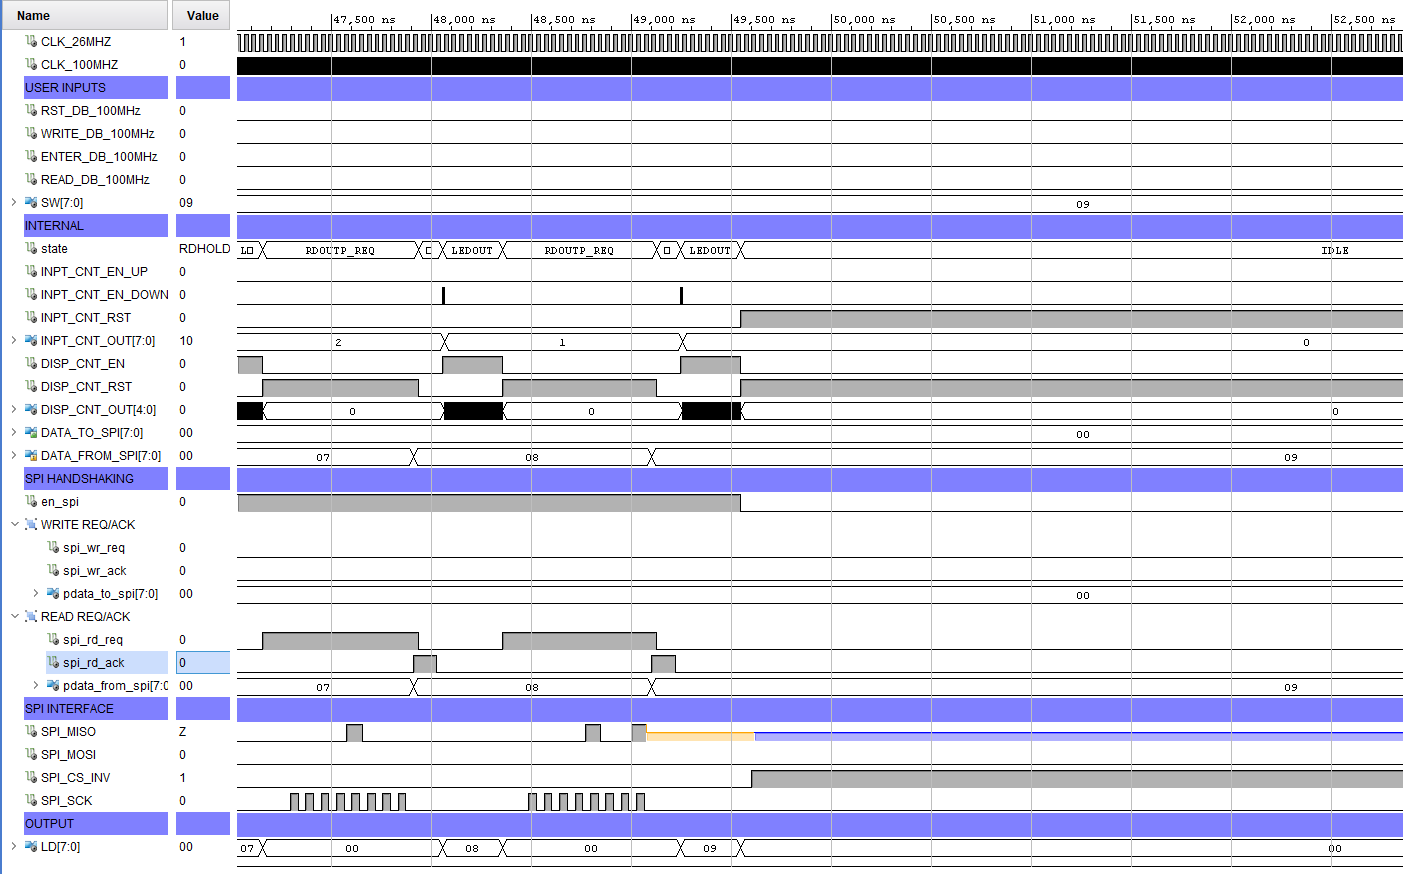
\includegraphics[width=\columnwidth]{Assets/Test6_3.PNG}
\end{figure}

The waveforms above show  the 10 stored (more than 0) switch values and exited `WRITE' mode in the previous test, the circuit should now be in `RDHOLD' state, waiting for the user to toggle the READ button. As soon as that button is toggled, the circuit should read and display the exact values that we're previously written, and should stop as soon as all values previously written have been displayed. This test will verify that the circuit can perform this function.

\subsection*{Log File: Test 6}
\begin{figure}[H]
    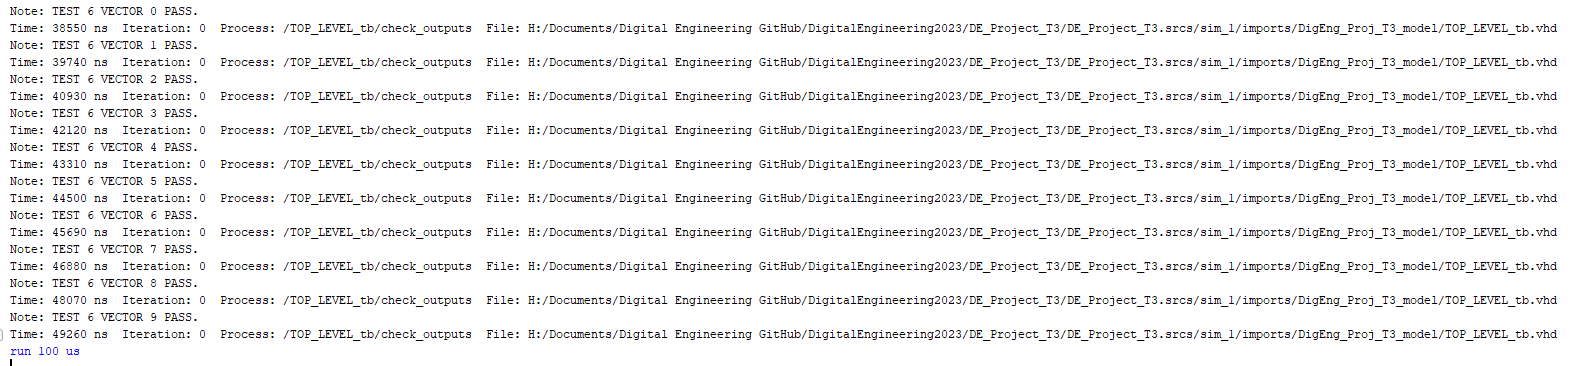
\includegraphics[width=\columnwidth]{Assets/Test6Console.PNG}
\end{figure}

Above shows the output of the self checking test for Test 6.

\section*{5 - ChipScope ILA Waveforms}

\subsection*{ILA Waveform of READ}
\begin{figure}[H]
    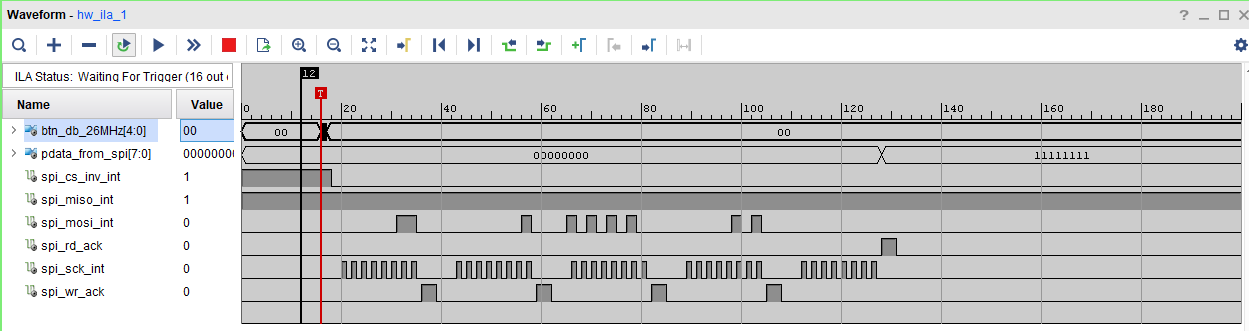
\includegraphics[width=\columnwidth]{Assets/ILA_read.PNG}
\end{figure}

Read mode is entered as the instruction is sent first (binary 3), the next three instructions are the memory address byte-by-byte (01, aa, 05). Finally, the logic will send a read request, which the waveform proves as we see a READ ACK.

Unfortunately for some reason, we couldn't figure out why the output wasn't working with the MISO line staying high even after the read ack, which was really abnormal. This caused our logic to output h'ff.

\subsection*{ILA Waveform of WRITE}
\begin{figure}[H]
    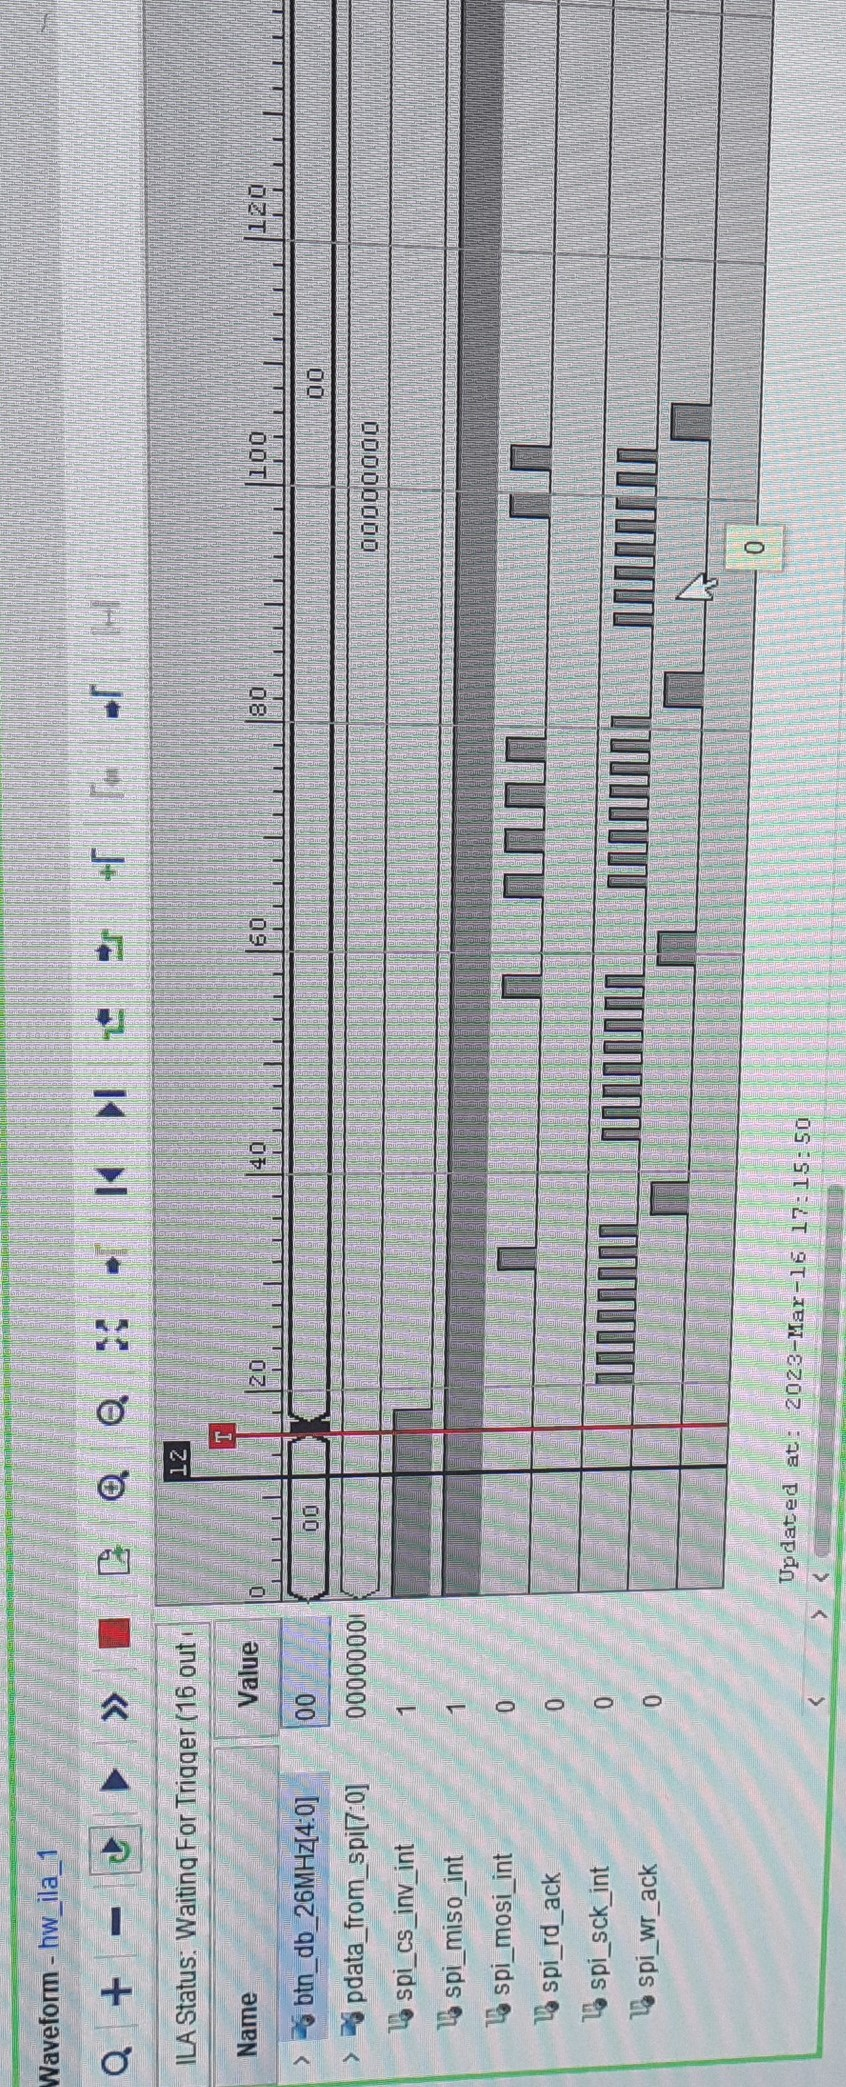
\includegraphics[angle=-90,origin=c,width=\columnwidth]{Assets/ILA_write.jpeg}
\end{figure}

The logic enters write mode with as the write instruction is first sent (binary 1), then 3 bytes of the address is also sent (01, aa, 05), each transmission followed by a write ack from the SPI. 

\subsection*{ILA Waveform of ENTER}
\begin{figure}[H]
    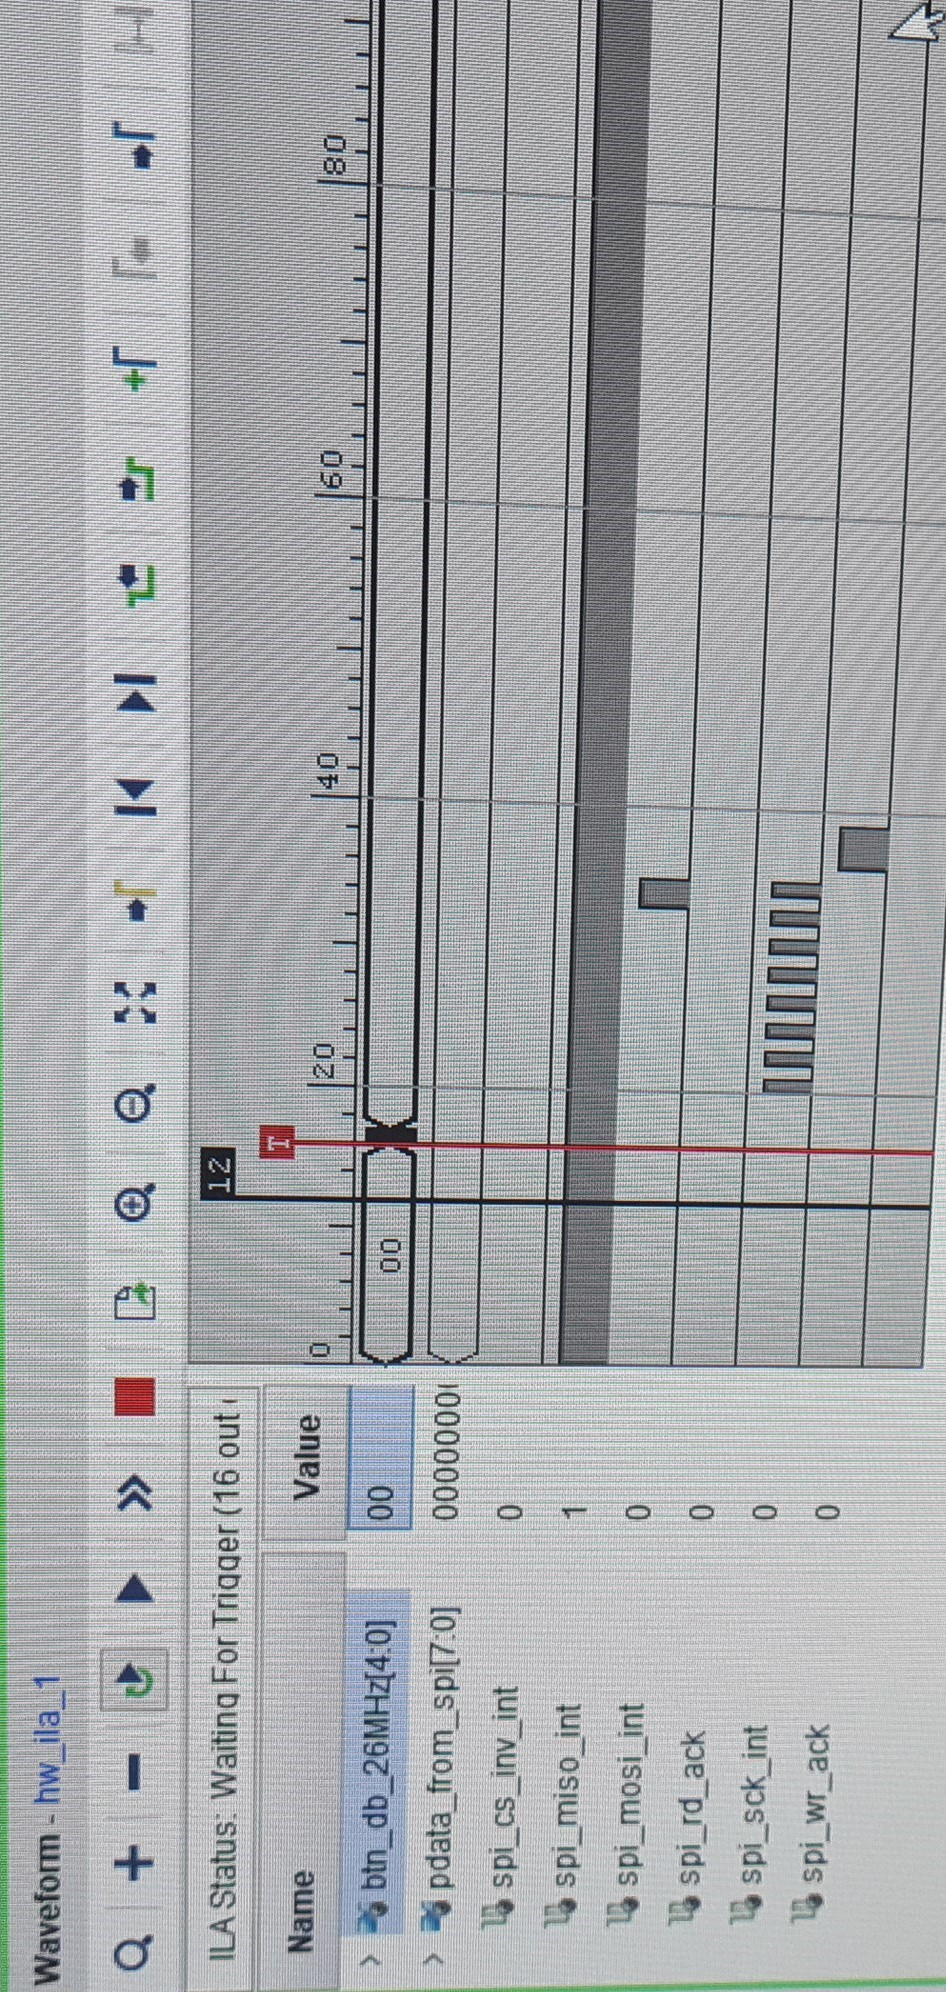
\includegraphics[angle=-90,origin=c,width=\columnwidth]{Assets/ILA_enter.jpeg}
\end{figure}

With the switches to binary 01 and pressing the ENTER button, we send that signal to the SPI, and SPI responds with a WR ACK.

\newpage

\section*{6 - Synthesis Report}

\subsection*{RTL Component Statistics}
\inputminted[firstline=213,lastline=236]{text}{../../../DE_Project_T3/DE_Project_T3.runs/synth_1/TOP_LEVEL.vds}

\newpage

\subsection*{RTL Hierarchical Component Statistics}
\inputminted[firstline=239,lastline=290]{text}{../../../DE_Project_T3/DE_Project_T3.runs/synth_1/TOP_LEVEL.vds}

\end{document}